\documentclass[11pt]{IEEEtran}
\usepackage{graphicx}
\usepackage{url}

\ifCLASSINFOpdf
  % \usepackage[pdftex]{graphicx}
  % declare the path(s) where your graphic files are
  % \graphicspath{{../pdf/}{../jpeg/}}
  % and their extensions so you won't have to specify these with
  % every instance of \includegraphics
  % \DeclareGraphicsExtensions{.pdf,.jpeg,.png}
\else
  % or other class option (dvipsone, dvipdf, if not using dvips). graphicx
  % will default to the driver specified in the system graphics.cfg if no
  % driver is specified.
  % \usepackage[dvips]{graphicx}
  % declare the path(s) where your graphic files are
  % \graphicspath{{../eps/}}
  % and their extensions so you won't have to specify these with
  % every instance of \includegraphics
  % \DeclareGraphicsExtensions{.eps}
\fi
% graphicx was written by David Carlisle and Sebastian Rahtz. It is
% required if you want graphics, photos, etc. graphicx.sty is already
% installed on most LaTeX systems. The latest version and documentation can
% be obtained at: 
% http://www.ctan.org/tex-archive/macros/latex/required/graphics/
% Another good source of documentation is "Using Imported Graphics in
% LaTeX2e" by Keith Reckdahl which can be found as epslatex.ps or
% epslatex.pdf at: http://www.ctan.org/tex-archive/info/
%
% latex, and pdflatex in dvi mode, support graphics in encapsulated
% postscript (.eps) format. pdflatex in pdf mode supports graphics
% in .pdf, .jpeg, .png and .mps (metapost) formats. Users should ensure
% that all non-photo figures use a vector format (.eps, .pdf, .mps) and
% not a bitmapped formats (.jpeg, .png). IEEE frowns on bitmapped formats
% which can result in "jaggedy"/blurry rendering of lines and letters as
% well as large increases in file sizes.
%
% You can find documentation about the pdfTeX application at:
% http://www.tug.org/applications/pdftex





% *** MATH PACKAGES ***
%
%\usepackage[cmex10]{amsmath}
% A popular package from the American Mathematical Society that provides
% many useful and powerful commands for dealing with mathematics. If using
% it, be sure to load this package with the cmex10 option to ensure that
% only type 1 fonts will utilized at all point sizes. Without this option,
% it is possible that some math symbols, particularly those within
% footnotes, will be rendered in bitmap form which will result in a
% document that can not be IEEE Xplore compliant!
%
% Also, note that the amsmath package sets \interdisplaylinepenalty to 10000
% thus preventing page breaks from occurring within multiline equations. Use:
%\interdisplaylinepenalty=2500
% after loading amsmath to restore such page breaks as IEEEtran.cls normally
% does. amsmath.sty is already installed on most LaTeX systems. The latest
% version and documentation can be obtained at:
% http://www.ctan.org/tex-archive/macros/latex/required/amslatex/math/





% *** SPECIALIZED LIST PACKAGES ***
%
%\usepackage{algorithmic}
% algorithmic.sty was written by Peter Williams and Rogerio Brito.
% This package provides an algorithmic environment fo describing algorithms.
% You can use the algorithmic environment in-text or within a figure
% environment to provide for a floating algorithm. Do NOT use the algorithm
% floating environment provided by algorithm.sty (by the same authors) or
% algorithm2e.sty (by Christophe Fiorio) as IEEE does not use dedicated
% algorithm float types and packages that provide these will not provide
% correct IEEE style captions. The latest version and documentation of
% algorithmic.sty can be obtained at:
% http://www.ctan.org/tex-archive/macros/latex/contrib/algorithms/
% There is also a support site at:
% http://algorithms.berlios.de/index.html
% Also of interest may be the (relatively newer and more customizable)
% algorithmicx.sty package by Szasz Janos:
% http://www.ctan.org/tex-archive/macros/latex/contrib/algorithmicx/




% *** ALIGNMENT PACKAGES ***
%
%\usepackage{array}
% Frank Mittelbach's and David Carlisle's array.sty patches and improves
% the standard LaTeX2e array and tabular environments to provide better
% appearance and additional user controls. As the default LaTeX2e table
% generation code is lacking to the point of almost being broken with
% respect to the quality of the end results, all users are strongly
% advised to use an enhanced (at the very least that provided by array.sty)
% set of table tools. array.sty is already installed on most systems. The
% latest version and documentation can be obtained at:
% http://www.ctan.org/tex-archive/macros/latex/required/tools/


%\usepackage{mdwmath}
%\usepackage{mdwtab}
% Also highly recommended is Mark Wooding's extremely powerful MDW tools,
% especially mdwmath.sty and mdwtab.sty which are used to format equations
% and tables, respectively. The MDWtools set is already installed on most
% LaTeX systems. The lastest version and documentation is available at:
% http://www.ctan.org/tex-archive/macros/latex/contrib/mdwtools/


% IEEEtran contains the IEEEeqnarray family of commands that can be used to
% generate multiline equations as well as matrices, tables, etc., of high
% quality.


%\usepackage{eqparbox}
% Also of notable interest is Scott Pakin's eqparbox package for creating
% (automatically sized) equal width boxes - aka "natural width parboxes".
% Available at:
% http://www.ctan.org/tex-archive/macros/latex/contrib/eqparbox/





% *** SUBFIGURE PACKAGES ***
%\usepackage[tight,footnotesize]{subfigure}
% subfigure.sty was written by Steven Douglas Cochran. This package makes it
% easy to put subfigures in your figures. e.g., "Figure 1a and 1b". For IEEE
% work, it is a good idea to load it with the tight package option to reduce
% the amount of white space around the subfigures. subfigure.sty is already
% installed on most LaTeX systems. The latest version and documentation can
% be obtained at:
% http://www.ctan.org/tex-archive/obsolete/macros/latex/contrib/subfigure/
% subfigure.sty has been superceeded by subfig.sty.



%\usepackage[caption=false]{caption}
%\usepackage[font=footnotesize]{subfig}
% subfig.sty, also written by Steven Douglas Cochran, is the modern
% replacement for subfigure.sty. However, subfig.sty requires and
% automatically loads Axel Sommerfeldt's caption.sty which will override
% IEEEtran.cls handling of captions and this will result in nonIEEE style
% figure/table captions. To prevent this problem, be sure and preload
% caption.sty with its "caption=false" package option. This is will preserve
% IEEEtran.cls handing of captions. Version 1.3 (2005/06/28) and later 
% (recommended due to many improvements over 1.2) of subfig.sty supports
% the caption=false option directly:
%\usepackage[caption=false,font=footnotesize]{subfig}
%
% The latest version and documentation can be obtained at:
% http://www.ctan.org/tex-archive/macros/latex/contrib/subfig/
% The latest version and documentation of caption.sty can be obtained at:
% http://www.ctan.org/tex-archive/macros/latex/contrib/caption/




% *** FLOAT PACKAGES ***
%
%\usepackage{fixltx2e}
% fixltx2e, the successor to the earlier fix2col.sty, was written by
% Frank Mittelbach and David Carlisle. This package corrects a few problems
% in the LaTeX2e kernel, the most notable of which is that in current
% LaTeX2e releases, the ordering of single and double column floats is not
% guaranteed to be preserved. Thus, an unpatched LaTeX2e can allow a
% single column figure to be placed prior to an earlier double column
% figure. The latest version and documentation can be found at:
% http://www.ctan.org/tex-archive/macros/latex/base/



%\usepackage{stfloats}
% stfloats.sty was written by Sigitas Tolusis. This package gives LaTeX2e
% the ability to do double column floats at the bottom of the page as well
% as the top. (e.g., "\begin{figure*}[!b]" is not normally possible in
% LaTeX2e). It also provides a command:
%\fnbelowfloat
% to enable the placement of footnotes below bottom floats (the standard
% LaTeX2e kernel puts them above bottom floats). This is an invasive package
% which rewrites many portions of the LaTeX2e float routines. It may not work
% with other packages that modify the LaTeX2e float routines. The latest
% version and documentation can be obtained at:
% http://www.ctan.org/tex-archive/macros/latex/contrib/sttools/
% Documentation is contained in the stfloats.sty comments as well as in the
% presfull.pdf file. Do not use the stfloats baselinefloat ability as IEEE
% does not allow \baselineskip to stretch. Authors submitting work to the
% IEEE should note that IEEE rarely uses double column equations and
% that authors should try to avoid such use. Do not be tempted to use the
% cuted.sty or midfloat.sty packages (also by Sigitas Tolusis) as IEEE does
% not format its papers in such ways.





% *** PDF, URL AND HYPERLINK PACKAGES ***
%
%\usepackage{url}
% url.sty was written by Donald Arseneau. It provides better support for
% handling and breaking URLs. url.sty is already installed on most LaTeX
% systems. The latest version can be obtained at:
% http://www.ctan.org/tex-archive/macros/latex/contrib/misc/
% Read the url.sty source comments for usage information. Basically,
% \url{my_url_here}.





% *** Do not adjust lengths that control margins, column widths, etc. ***
% *** Do not use packages that alter fonts (such as pslatex).         ***
% There should be no need to do such things with IEEEtran.cls V1.6 and later.
% (Unless specifically asked to do so by the journal or conference you plan
% to submit to, of course. )


% correct bad hyphenation here
\hyphenation{op-tical net-works semi-conduc-tor}


\begin{document}
%
% paper title
% can use linebreaks \\ within to get better formatting as desired
\title{A Peer-to-Peer Personal Storage System}


% author names and affiliations
% use a multiple column layout for up to three different
% affiliations
\author{\IEEEauthorblockN{Adrien Ecoffet}\\
\IEEEauthorblockA{
adrien.ecoffet@gmail.com}\\
\&\\
\IEEEauthorblockN{Fabrice Bascoulergue}\\
\IEEEauthorblockA{
f.bascoulergue@gmail.com}}

% conference papers do not typically use \thanks and this command
% is locked out in conference mode. If really needed, such as for
% the acknowledgment of grants, issue a \IEEEoverridecommandlockouts
% after \documentclass

% for over three affiliations, or if they all won't fit within the width
% of the page, use this alternative format:
% 
%\author{\IEEEauthorblockN{Michael Shell\IEEEauthorrefmark{1},
%Homer Simpson\IEEEauthorrefmark{2},
%James Kirk\IEEEauthorrefmark{3}, 
%Montgomery Scott\IEEEauthorrefmark{3} and
%Eldon Tyrell\IEEEauthorrefmark{4}}
%\IEEEauthorblockA{\IEEEauthorrefmark{1}School of Electrical and Computer Engineering\\
%Georgia Institute of Technology,
%Atlanta, Georgia 30332--0250\\ Email: see http://www.michaelshell.org/contact.html}
%\IEEEauthorblockA{\IEEEauthorrefmark{2}Twentieth Century Fox, Springfield, USA\\
%Email: homer@thesimpsons.com}
%\IEEEauthorblockA{\IEEEauthorrefmark{3}Starfleet Academy, San Francisco, California 96678-2391\\
%Telephone: (800) 555--1212, Fax: (888) 555--1212}
%\IEEEauthorblockA{\IEEEauthorrefmark{4}Tyrell Inc., 123 Replicant Street, Los Angeles, California 90210--4321}}




% use for special paper notices
%\IEEEspecialpapernotice{(Invited Paper)}




% make the title area
\maketitle


\begin{abstract}
Personal storage services have become increasingly popular in recent years, with services like Dropbox, Google Drive, Microsoft Skydrive or Apple iCloud\cite{dropbox, drive, skydrive, icloud}. Because these services, by and large, are used to synchronize personal files across devices rather than to increase one's available storage space, it appears possible to devise a system in which users would share some of their existing disk space to be able to store files in the cloud for free.

We propose a purely distributed peer-to-peer solution to that problem, and examine some of the challenges such a solution must face. We then present Jellyfish, our prototype for such a system, and the results of performance tests on a small cluster of Jellyfish instances.
\end{abstract}

\section{Introduction}

File synchronization services are more popular than ever today. This is in large part due to the increasing number of computing devices people have in their possession. On the other hand, commodity hard drives can now store huge amounts of data (typically 500GB to 2TB). Those two facts make it possible to design a system that would use unused space on user hard drives to provide an amount of cloud storage space proportional to the amount shared to the network by the user. 

The system would store encrypted versions of the files on other users' filesystems so that files can be retrieved at any point in time by the user.

\subsection{Related Work}

Some similar systems have already been proposed. Clearly this somewhat resembles some distributed file systems, especially those that support disconnected operations, such as Coda\cite{coda}, but some even more similar commercial services have also been created.

The first of them was probably Wuala\cite{wuala:measurement}, which initially featured a way to increase one's available storage space by sharing some disk space. Note that all files were still stored on their servers and that this was only used to increase performance. The feature has since been dropped.

Another example is SpaceMonkey\cite{spacemonkey}, which allows users to rent large hard drives that are constantly connected to the Internet and are part of a peer-to-peer network which stores other user's files.

Very recently, Bittorrent announced Bittorrent Sync\cite{sync}, which is very similar to our proposal. The differences we have seen are the following: Bittorrent Sync doesn't have a notion of an user account, rather users are expected to share a secret key across their devices. Additionally, Bittorrent doesn't ask the user how much of their hard drive it should share. It is unclear exactly how it determines that. Bittorrent Sync is also tracker-based, while our proposal is fully decentralized. Most importantly, Bittorrent hasn't released any paper or source code that we know of so far.

A company called Maidsafe is apparently currently developing a peer-to-peer system very similar to ours\cite{maidsafe_site}, but it hasn't been released so far. However, Maidsafe has developed and released an implementation of the Kademlia distributed hash table\cite{maidsafe_dht} which we use in our implementation (its convenience is understandable since it was developed for this purpose exactly).

\section{Efficient storage}

It should be quite clear that the chances of failure of any given node are quite high in such a network, since real world computer users generally don't have their computers turned on at all time. As far as metadata is concerned, we choose to use an existing distributed hash table implementation (in our case Maidsafe-DHT, an version of Kademlia). However, it would be impossible to store files, especially large ones, directly in the DHT, partly because of performance reasons (we want to get several parts of the files from different nodes so as to maximize network performance), and mostly because replication in DHTs isn't suited to large files: our particular implementation stores 4 instances of any value in the DHT and proactively transfers the value to other nodes when one of the nodes involved in storing it goes down. Besides, Maidsafe-DHT is a fully in-RAM implementation, so it couldn't sustain a large amount of data.

There must therefore be a ratio between the space a user allocates on her hard drive and the amount of data she is able to store on the network, with the former value being likely higher than the latter. What follows is a set of techniques that can be used to bring that ratio as close to 1 as possible.

\subsection{Avoiding Best Fits}

A common technique employed by companies in the personal cloud storage industry is to make it hard for users to get an amount of storage space that actually fits their needs. For example, Dropbox proposes either 2GB, 100GB, 200GB or 500GB of storage for individuals\cite{dropbox}, which makes it hard to find a type of account that actually fits the exact need of an individual user. What this means is that users who are underusing their Dropbox account are actually paying for the ones that are using theirs to its fullest.

We believe it is useful to make sure that users can only choose their amount of storage space from a set of exponentially growing possible sizes. This way the network would be able to do more replication than seemingly implied by the ratio, because the network will be underused.

Our implementation uses powers of two as a simple exponentially growing set of size choices, but it is probable that a real world system would grow even faster, like Dropbox.

Data released by Dropbox in 2011 indicates users were storing on average 400MB in their Dropbox\cite{dropbox_slides}, which tends to confirm that using exponentially increasing storage options is a good way to get the service to be underused.

\subsection{Compression}

Compression seems like an obvious solution, although in practice it might not be that useful since users are likely to store compressed media files such as MP3 audio files, or even PDF files. These files do not compress very well at all, however, it seems that compressing them using gzip will still often make them 1\% or 2\% smaller\cite{compression_comparison}, so compression certainly doesn't hurt, which is why we included it in our pipeline.

Gzip compression is commonly used in other Internet transmissions and is currently much faster than the typical bandwidth of a personal computer, so it won't be a bottleneck.

\subsection{Erasure Coding}

Erasure codes (such as Reed-Solomon codes) allow for generating $n$ parts and $m$ error codes and for reconstructing the file if any $n$ of the $n + m$ blocks are fetched from the network. This greatly increases the probability of retrieving a file since, for sufficiently large $n$, the replication ratio $n/(n+m)$ only has to approximate the probability of any given node being online. 

We use the Jerasure implementation of Cauchy Reed-Solomon codes, which seem to be the fastest open-source implementation of general purpose erasure codes\cite{comparison_reed_solomon}. 

It is to be noted that because we can only split a file into a discrete and relatively small number of parts and codes for performance reasons: there is overhead involved in creating more parts and codes, because generating codes involves padding, and using more parts will generally mean more of it overall, because generating more parts will generally take more CPU power, and finally because it will involve making more connections to nodes, which means more network overhead.

This and the fact that the number of reachable nodes at any given time might be lower than the uptime ratio would predict, and, when the network is initially small, might not even be sufficient to store each file block on a different node, combine in way that means that the ratio of code blocks / total blocks must be higher than the estimated average uptime ratio of the network. We made several simulations to understand the way the probability of recovering files evolves according to these parameters.

Figure 1 shows how the total number of nodes in the network can influence the probability of recovering a file for small networks. We can see that the negative influence of a small number of nodes is significant. Like all other simulations here, it was done with 5,000 samples. 

Figure 2 shows how the proportion of codes to the total number of blocks, i.e. the replication ratio influences the probability of recovering a file. Because we assume roughly 66\% average uptime across the network, we have decided to use 10 parts and 13 codes based on this graph. Clearly this is not ideal because the probability of retrieving a file is not 100\% in this case, but this allows our tests to more clearly show the improvement as the network grows larger.

Figure 3 shows the probability of recovering a file as a function of the absolute number of parts, with a replication ratio of 2 codes per part.

\begin{figure}
\centering
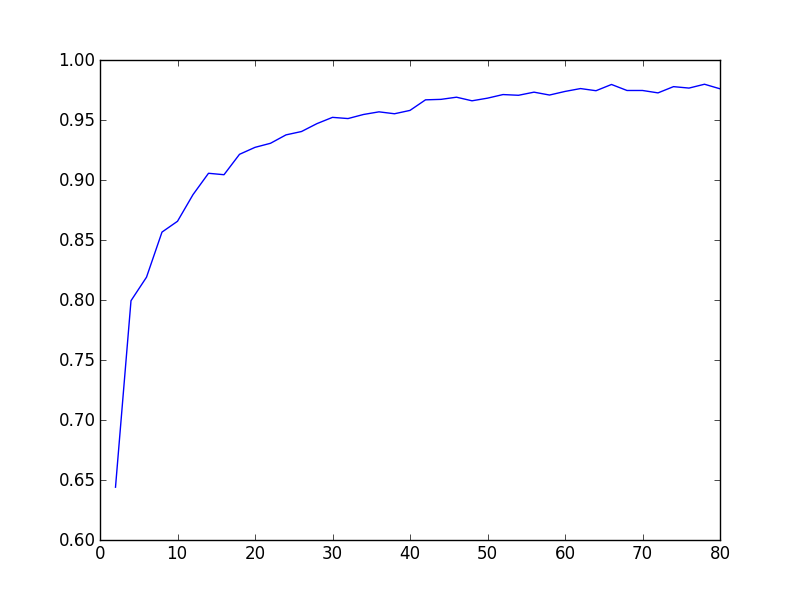
\includegraphics[scale=0.43]{test.png}
\caption{Simulated probability of recovering file as a function of the number of nodes: 10 parts, 13 codes, 66\% uptime}
\end{figure}
\begin{figure}
\centering
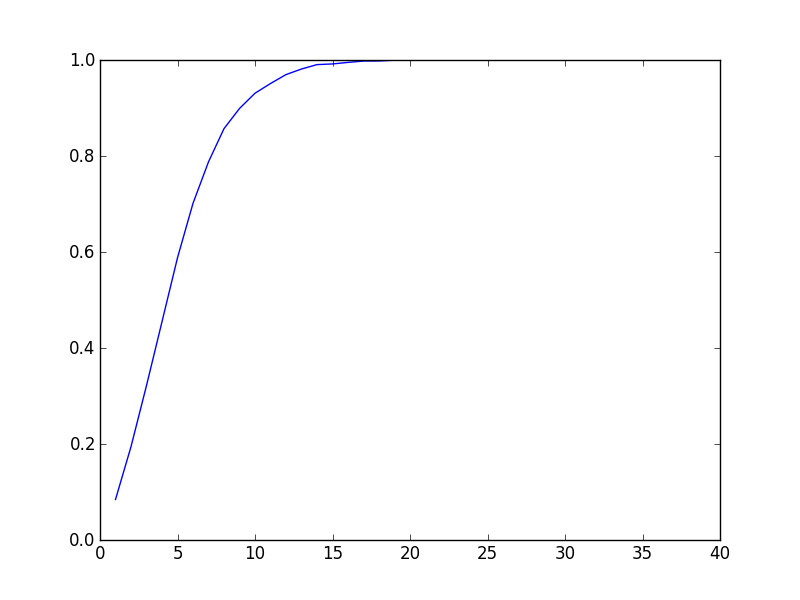
\includegraphics[scale=0.43]{test2.png}
\caption{Simulated probability of recovering file as a function of the number of codes: 10 parts, 66\% uptime, 100 nodes}
\end{figure}
\begin{figure}
\centering
\includegraphics[scale=0.43]{test3.png}
\caption{Simulated probability of recovering file as a function of the number of parts, with a ratio of 2 codes for each part: 60\% uptime, 50 nodes}
\end{figure}

\subsubsection{Overhead}

As mentioned, erasure codes do have some overhead due to padding, which is used to make the file size a multiple of the size of the buffer used to generate the codes. A larger buffer generally means that the codes will be generated more quickly (although this fails for very large buffer because of bad cache behavior), a smaller buffer generally means that the padding will be lower. We chose to compute a good buffer size based on the actual size of the file, trading off speed for a lower buffer size if necessary, and using a large buffer when the file size is close to a multiple of a large enough buffer.

Because erasure coding is done after compression and encryption in our case, it is unfortunately necessary to wait at least for compression to finish to get the size of the file to erasure-code. This is unfortunate as it makes it impossible to run the whole pipeline in parallel. We didn't focus too much on such performance issues, but it might be necessary for production systems to hardcode a reasonable buffer size in order to compress, encrypt, erasure-code and send the file blocks all in parallel. 

Because of the overhead involved, we also chose to store small files (less than 100KB in our case) directly inside the DHT. This is because for small files the overhead can be of more than 100\%, which we really don't want.

Another way to fix the small files problem would be to bundle several small files into one larger archive, an area future work could investigate.

\subsection{Pipeline}

Several pipelines are possible for this system. The elements of the pipeline would be compression, erasure coding and encryption. Clearly encryption cannot take place before compression because encrypted data almost never compresses at all. It is possible to compress Cauchy Reed-Solomon codes to some extent if they weren't created from encrypted data, but experiments we made show that they compress significantly less well than the original file, so clearly compression should be the first step. There is no significant difference between encrypting after creating erasure codes or before that, apart from the fact that the total amount of data to encrypt will be significantly higher if erasure coding is done first. This leads us to our final pipeline (shown in Figure 4): compression, then encryption, then erasure coding.

\begin{figure}
\centering
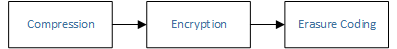
\includegraphics[scale=0.8]{flow1.png}
\caption{Our chosen pipeline}
\end{figure}

As we have mentioned, our pipeline doesn't run fully in parallel, but it is clear that if it were we'd be seeing a speed of data generation higher than the upload bandwidth of the vast majority of individual users (our estimate is that the generation speed of a fully parallel pipeline would be around 50MB/s).

Additionally, our implementation transfers data using thrift for simplicity, which means that sending and receiving data is a fundamentally synchronous operation and cannot happen as the last or first part of a real pipeline. Obviously a production implementation would use network streams instead of RPC and could thus take advantage of the pipeline.

\section{Threat Model}

A major issue in a decentralized system like this one is that of security. Here we consider the security of our design against three types of attackers: eavesdroppers, economically motivated attackers (cheaters) and Byzantine attackers.

\subsection{Eavesdroppers}

Eavesdroppers want to access user data, i.e. steal user files, steal user accounts, get some knowledge of exactly what files a given user has etc.

We simply use the typical way to protect oneself against eavesdropper: cryptography is used extensively in the system. User are each assigned a RSA private key which identifies them. The vast majority of operations require a signature from the user. Users also have a single AES256 key which is stored in the distributed hash table, encrypted using the user's public key (this is because AES cryptography is much faster than RSA). All files are encrypted using this AES key and a separate random IV. Some private user data is stored that way as well. Note that a separate key could also be used for each file, though this would incur a slight performance penalty.

Because we want to provide the abstraction of a user account rather than require users to transfer their private keys across their devices, private keys are actually store in the DHT, encrypted using an AES256 key that is derived from the user "password" using PBKDF2\cite{PBKDF2} (note: a better alternative for a production system could be scrypt\cite{scrypt}, but PBKDF2 implementations are more widely available). This clearly makes the system vulnerable to dictionary attacks on passwords, so a real system should probably have a password strength verification module and should educate users about the importance of a strong password, especially in this context.

Note that an alternative would have been to generate the private key directly from the password using PBKDF2, but that would have made it extremely hard for users to change their passwords later.

Additionally, the DHT we chose to use uses public key cryptography to ensure that, for instance, nodes which do not have a user's private key are unable to delete or modify values that have been set by that user. 

\subsection{Cheaters}

Cheaters are economically motivated attackers.

An important concern in such a system as ours is the possibility of having users that use the file synchronization service without actually sharing the right amount of space to the network. The two main ways to do this would be to only connect to the network to perform actions such as storing and downloading files, or simply not actually storing the file blocks one is in charge of. 

\subsubsection{\textbf{Karma}}

Misbehaving nodes accumulate karma. When a node finds another node is misbehaving, it adds a karma record to the node's public karma set. Karma records exist for a limited amount of time (30 days in our current implementation) and contribute to diminishing the node's contribution to the user's overall allowed amount of storage.

For instance, if a node is found not to be connected at a given time, a NotConnected karma record will be added to it. These NotConnected records are then used to estimate the uptime of the node during the last 30 days, and the node's contribution to the overall allowed storage space for the user will be proportional its uptime. Since there is a linear relation between uptime and available storage space (0\% uptime will mean that the node doesn't contribute to the user available storage, 100\% contributes the maximum possible value), there is always an incentive for nodes to remain connected.

As another example, if a node is found to be connected but fails to prove that it does indeed store a good version of a given file part, a DeletedPart karma record will be associated with it. While it is normal for a node to be disconnected at some point, deleting a file part is considered explicitly malicious behavior and is thus harshly punished. In our implementation, three DeletedPart records within a month bring the user's allowed storage space down to 0. Unlike with disconnected nodes, the specifics of the punishment don't matter too much here, as long as they create a strong incentive to keep the file blocks.

Our implementation of the storage system does find cheaters with high probability, although this clearly depends on the amount of cheating: a user could reasonably get away with deleting a single block from her disk for a fairly large amount of time, but the really useful form of cheating that consists in deleting large amounts of data is generally caught within a few hours in our implementation that sends a challenge every ten minutes on average.

\subsubsection{Random Threats}

An issue with this system is that these errors are ordinarily detected only when a client tries to download a file, which is a fairly uncommon event.

For this reason, every online client will regularly keep a check on their file blocks by doing the following: when a file is added, the client generate hashes for each file block using different random salts. Then the client will regularly and randomly require nodes that store blocks from its files to compute the hash of one of their blocks using a salt they have never seen before. If the node computes a correct hash, it can be assumed that it still has the file block. If the client runs out of precached hash challenges it can always recreate a few from the files it still has locally.

It should be clear that nodes shouldn't be able to generate a correct hash of the file with a new salt (all salts in our implementation are 128 bits, which would make storing a lookup table extremely expensive, especially when it would likely be bigger than the file part) if they do not actually have the file, as this would constitute a collision attack on the hash function (SHA-256 in this case), which we assume is impossible.

\subsection{Byzantine Attackers}

Byzantine attackers could exploit issues with the system for no apparent reason. One such issue which is intrinsic to using a DHT is the Sybil attack\cite{sybil}, but it is definitely out of the scope of this project. 

Another thing a Byzatine attacker might do is trying to delete data from the DHT. Fortunately, Maidsafe-DHT will allow such operations to be performed only by nodes which have the same private key as the node which initially set the value in the DHT, so this would be impossible.

Yet another is to add karma records to other nodes to reduce their maximum storage space. Unfortunately we haven't found a way to prevent this issue that would still make it possible to catch misbehaving nodes and that would be efficient, since any such method would require the help of a third party. We chose not to handle these attacks in our system. Presumably that means that users should keep their usernames secret so as to be less likely to be considered targets by such attackers. Maybe a better solution could be found in future work.

\section{Future Features}

These are features that we believe can be added to similar systems in a fairly straightforward manner, but that we didn't implement because our focus in our implementation was to create a proof of concept and not a production-ready system.

\subsection{File Sharing}

A common feature of file storage services is sharing files among user, which is particularly useful in an enterprise context. 

The way this can be done in a network such as ours is by having each file have a separate AES256 key (in our current implementation each user has a global AES256 key and each file only has a unique initialization vector), and creating a notion of user groups. Each group also has a separate key which allows members of the group (who have the key) to decrypt and use the individual file keys which are stored encrypted inside of the DHT.

An alternative would be to use the group key directly to encrypt the file, but we suspect changing the sharing preferences of a file would be a very common operation, and by adding a level of indirection by encrypting the keys instead of the files using the group key, moving a file from one group to another becomes a much more lightweight operation.

An inconvenient of doing this is that it causes additional overhead on the DHT and while fetching a file that is shared, but this should be negligible.

\subsection{Duplicate Merging}

A way all commercial services reduce the amount of data they actually need to store is by merging duplicate files.

If two users upload the same file, it shouldn't be necessary to store the file twice. This way less data has to be actually stored, and upload can be made instantaneous for files which are duplicates of other files on the network, under some implementations.

Implementing this feature on a centralized service is straightforward: when the file is uploaded, a hash of it is computed and if it is the same as one already stored in the system, the uploaded data is simply dropped. In a decentralized system like ours, however, the problem gets trickier: it mustn't be possible for a user to obtain the encryption key to a given file simply by saying they already have a version of it, as this would be a huge infringement of anonymity.

There are two ways this could be solved: one way would be for the user to contact a node belonging to the user which has the original file, send it the whole file and have that user check if the file is indeed correct. If it is, the user can then send back its encryption key for the file and then both users would be able to access the same file.

This approach has a few problems though: for one, it requires the first owner of the file to be connected at this time. It is expensive in terms of CPU and bandwidth for both users and it does not allow for the optimization that consists in not ever uploading the file.

Another, much better approach would be this: when a user first uploads a file, it stores it under a key that corresponds to the file's unsalted hash. In the file record it stores a random salt, and then generates the encryption key from a hash of the salt concatenated with the file. When a new user wants to upload the file, it looks it up in the DHT, and if it finds a record, computes the same salted hash to get the encryption key, and then stores it in a private way.

This method guarantees that only a user that possesses a given file can obtain the encryption key, it can be done at any given time independent of other nodes in the network, and most importantly perhaps, allows for not actually uploading the file if it already exists (the user might want to download the file to check that its encryption key is correct, but there are other ways of doing this, such as storing known data encrypted using the key inside of the existing file record).

It might be useful to slow down the computation of the encryption key using a method similar to PBKDF2, where the number of iteration would be inversely proportional to the size of the file. This is mostly for very small files on which a brute force attack would be feasible.

A problem with those techniques is that it might be possible for an attacker to know which users possess a given file by knowing its hash. This is certainly an issue with the first approach, but we believe the second can be implemented in a way that does not reveal that information.

\subsection{Diffs and Versioning}

Updating a file currently consists in deleting it and adding it again. In practice however, uploading modifications to files can be made faster by sending diffs instead of complete new versions of the file. We haven't experimented with that topic, but we suspect it should be fairly easy to generate diffs and store them just like any other file on the network. Fetching the file would then require getting the old file and the diffs, and presumably diffs should be collapsed into the file regularly for download performance to remain good.

This is certainly an area a real world system could investigate. It would also make it trivial to provide a feature to fetch an old version of any given file, which some users might find useful.

\subsection{Streaming}

Our current implementation is blocking as far as receiving and sending the files is concerned: only Gzip compression/decompression and AES256 encryption/decryption are done concurrently. However, as discussed earlier, it is perfectly possible, and in fact trivial, to have a fully parallel pipeline that downloads, erasure-decodes, decrypts and decompresses at the same time (and vice versa for upload), which in the case of download would make it possible to stream media files directly from the synchronized storage.

A similar feature has been implemented in a peer-to-peer context by the uTorrent Bittorrent client.

\section{Tests}

We implemented a version of our storage system as described in this paper, which we called Jellyfish.

We used Amazon EC2 to run our tests on a sufficient number of nodes and get relevant results on two main points, the success probabilities of get and put operations and the CPU used by the software running as a background task. We did not measure bandwidth usage, but it can reasonably be assumed that DHT activity is negligible, and therefore that our bandwidth usage is roughly that of any other cloud storage service times the replication factor. We simulated clients connecting and disconnecting regularly and randomly over a defined period of time to create a non stable environment for our network.

\subsection{Success probabilities}

In this section, we will describe the probability of successfully storing a file in our system and retrieving it at different times.

This test as been done with our unstable nodes that remained connected twice as long as disconnected on average (with some randomness), i.e. the average uptime of the network was supposed to be 66\%.

We ran this test over four different networks, with 25, 50, 75 and 100 nodes.

Statistics for the "put" operation (storing a file) are shown by Figure 6. This operation gives really good results even with a very small network and almost give perfect results on the larger one. Those results were expected because the operation of storing a file can only fail if almost all the nodes decide to disconnect in the same period of time. So, increasing the number of node reduces the probability to find a case where all the nodes are disconnected at the same time and by induction increase the probability to have enough nodes to store a file.

Figure 7 shows the statistic for the "get" operation (retrieving a file). The probabilities for this operation to succeed are hard to predict because they mainly depend of the number of replicas, the availability of the nodes and the chance to find the nodes storing parts of this file. At a high level of implementation, it is definitely possible to compute this probability and to increase it by gathering informations about each node with their general availability (when is this node connected most often) and bandwitdth.

With our implementation and using our unstable network, this operation cannot give a success of 100\% because it is impossible to ensure that the minimum number of node(storing parts of this file) required to retrieve it will be connected during the operation. Also, we used 26 blocks for storing the file on the network so 25 nodes is not enough to give good results this is why the probability with this network is really low. From 50 nodes, we started to have enough nodes to ensure a good probability to have enough retrievable parts of the file. The network with 75 and 100 nodes increased this probability, however, even a network containing a thousand nodes would not increase this probability to 100\% because the number of parts would be too low to increase the availability of the file. It could be achieve by also increase this number of parts. 

Note that on this aspect our network seems to perform less well than the simulation from Figure 1. We believe this is mostly due to the fact that the actual average uptime of our network was actually slightly lower than 66\%. This is because program initialization, which can take about ten seconds wasn't counted as part of downtime. Since the nodes weren't very long running our tests (about 6 minutes on average), this can be fairly significant. Not to mention the fact that they might have been doing other work at different times (such as computing hashes for random threats), which would have made them unavailable for a couple seconds at a time. 

\subsection{CPU usage}

As mentioned before, the CPU utilization shown in Figure 5 comes from nodes with the software running as a background task. We did not include the "put" and "get" operations in the statistics because those operations use encryption and compression algorithms that are very expensive in terms of CPU usage and we think that the idle state is more important in terms of user experience: a user might expect the program to use resources when performing an explicit action, but the idle CPU use should be minimal. 

During idle state, the CPU is used mainly for two operations, namely storing a part and the "random threat", which both compute a hash. The operation of getting a part has a very small impact on CPU usage because it only needs to read and send this part.

The average CPU utilization computed over 20 nodes is 1.31\%. It appears that our goal to consume a small amount of cpu while idle is achieved.

\begin{figure}
\centering
\includegraphics[scale=0.43]{cpu.png}
\caption{Histogram of the CPU usage (in percentage) of idle nodes}
\end{figure}

\begin{figure}
\centering
\includegraphics[scale=0.43]{prob2.png}
\caption{Probability of a put request succeeding as a function of the number of nodes (samples: 25, 50, 75, 100)}
\end{figure}

\begin{figure}
\centering
\includegraphics[scale=0.43]{prob.png}
\caption{Probability of a get request succeeding as a function of the number of nodes (samples; 25, 50, 75, 100)}
\end{figure}

\section{Conclusions}

Our project demonstrates, successfully we believe, the feasibility of fully distributed peer-to-peer storage systems, such as streaming, duplicate merging, reliability, file sharing... We described ways to implement most features of commercial centralized cloud storage systems in a purely distributed fashion. We implemented a prototype of such a system and showed that it was viable and could be quite reliable. We introduced security issues such as cheating and proposed incentive-based solutions to them. We demonstrated that our software doesn't use too many resources when idle and would thus be suitable for everyday use.

There are many unimplemented features in our system and Jellyfish is thus not production ready, but we believe we have described ways to design  missing features fairly comprehensively which should help future work.
%\end{document}  % This is where a 'short' article might terminate

%ACKNOWLEDGMENTS are optional
\begin{thebibliography}{1}
\bibitem{dropbox} \url{http://dropbox.com}
\bibitem{drive} \url{http://drive.google.com}
\bibitem{skydrive} \url{http://skydrive.live.com}
\bibitem{icloud} \url{http://icloud.com}
\bibitem{wuala:measurement} Mager, Biersack, Michiardi, \emph{A measurement study of the {W}uala on-line storage service}, 2012
\bibitem{sync} \url{http://labs.bittorrent.com/experiments/sync.html}
\bibitem{spacemonkey} \url{http://spacemonkey.com}
\bibitem{maidsafe_site} \url{http://maidsafe.net}
\bibitem{maidsafe_dht} \url{https://code.google.com/p/maidsafe-dht/}
\bibitem{coda}  Kistler, Satyanarayanan, \emph{Disconnected operation in the Coda File System}, 1992
\bibitem{dropbox_slides} Houston, \emph{Dropbox startup lessons learned 2011}, 2011
\bibitem{compression_comparison} \url{http://bashitout.com/2009/08/30/Linux-Compression-Comparison-GZIP-vs-BZIP2-vs-LZMA-vs-ZIP-vs-Compress.html}
\bibitem{comparison_reed_solomon} Plank, \emph{A Performance Evaluation and Examination of Open-Source Erasure Coding Libraries For Storage}, 2009
\bibitem{PBKDF2} IETF, \emph{PKCS \#5: Password-Based Key Derivation Function 2 (PBKDF2) Test Vectors}, 2011
\bibitem{scrypt} Percival, \emph{Stronger Key Derivation via Sequential Memory-Hard Functions}, 2009
\bibitem{sybil} Douceur, \emph{The Sybil Attack}, 2002
\end{thebibliography}


% that's all folks
\end{document}


